% !TEX root = ../report.tex
\chapter{Konzept}
\begin{Spacing}{\mylinespace}

Wie bereits in der Einleitung angeführt, soll eine Strömungssimulation erarbeitet werden. Die Grandlage hierfür bilden zwei optische System. Im ersten Teil wird die Oberfläche mit einer Tiefenkamera eingelesen. Der zweite Teil besteht aus einem Projektor, welcher die simulierte Strömung direkt auf die eingelesene Oberfläche projeziert. Dies soll in Echtzeit erfolgen. Als Kernstück soll mit einem Rechner gearbeitet werden, auf dem die Simulationssoftware ausgeführt wird und alle optischen Systeme angebunden sind.

\section{Der Datenfluss}
Der Datenfluss unseres Projektes  wird in Abbildung \ref{fig:dataFlow} dargestellt. Zu Begin wird ein Tiefenbild mit der Kinekt erfasst und an die Simulationssoftware übermittelt. Die Anwendung verarbeitet die erfassten Daten und bereitet diese für die GPU vor. Anschließend arbeitet die GPU auf den erfassten Daten und erzeugt ein Bild welches abschließend über den Projektor ausgegeben wird.

\begin{figure}[h!]
	\centering
	\vspace*{20px}
	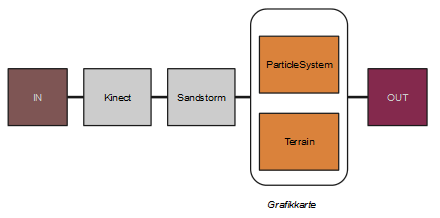
\includegraphics[width=0.6\textwidth]{graphics/flow.png}
	\caption{Datenfluss}
	\label{fig:dataFlow}
\end{figure}

\section{Die Modularisierung}
Um eine parallele Entwicklung und spätere Erweiterbarkeit sicherzustellen soll modulbasiert entwickelt werden. Das Projekt lässt sich in drei Kategorien gliedern. Bestandteile sind das ParticleSystem (ParticleSystem), die Kinect Ansteuerung (SandstormKinect) und einen Controller (Sandstorm), welcher Events entgegen nimmt und für die Verarbeitung zuständig ist. Die Basis bildet die DrawableGameCompontent, welches jeder Komponente einen eigenen Kontext zuweist. Dies bedeutet das jede DrawableGameCompontent ein separates Projekt darstellt und unabhängig betrieben werden kann. Die Strukturierung ist in Abbildung \ref{fig:singleColor} dargestellt.

\begin{figure}[h!]
	\centering
	\vspace*{20px}
	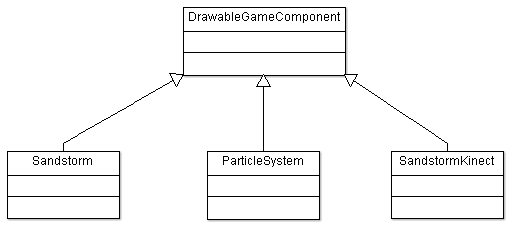
\includegraphics[width=0.6\textwidth]{graphics/DrawableGame.png}
	\caption{Kompontenten}
	\label{fig:singleColor}
\end{figure}

\section{Die Component Properties} \label{PropSec}
Um das  System so dynamisch wie möglich zu gestalten, sollen Sammelcontainer für Systemparameter einzuführt werden, sogenannte Properties.
Diese Properties sind vergleichbar mit Konfigurationsdateien. Ändert man einen Wert innerhalb einer Properties so wird der neue Wert sofort vom restlichen System übernommen. Für jede Kategorie (Physikengine,RenderEngine,Kinect..) soll ein solcher Container genutzt werden, um für verschiedene Anwendungscenarien Default-Wert zu hinterlegen und diese bei Bedarf zu laden oder zu speichern. Zusätzlich ermöglichen diese, die Erzeugung eines komplett dynamischen User Interface (s. Abschnitt \ref{GUISec}).

\end{Spacing}
\newpage
\clearpage
%% End Of Doc